\begin{figure}
  \centering
\fbox{
  \setlength{\unitlength}{\textwidth}
  \begin{picture}(0.6,0.5)

  
    % % %90
      \put(-0.1,0){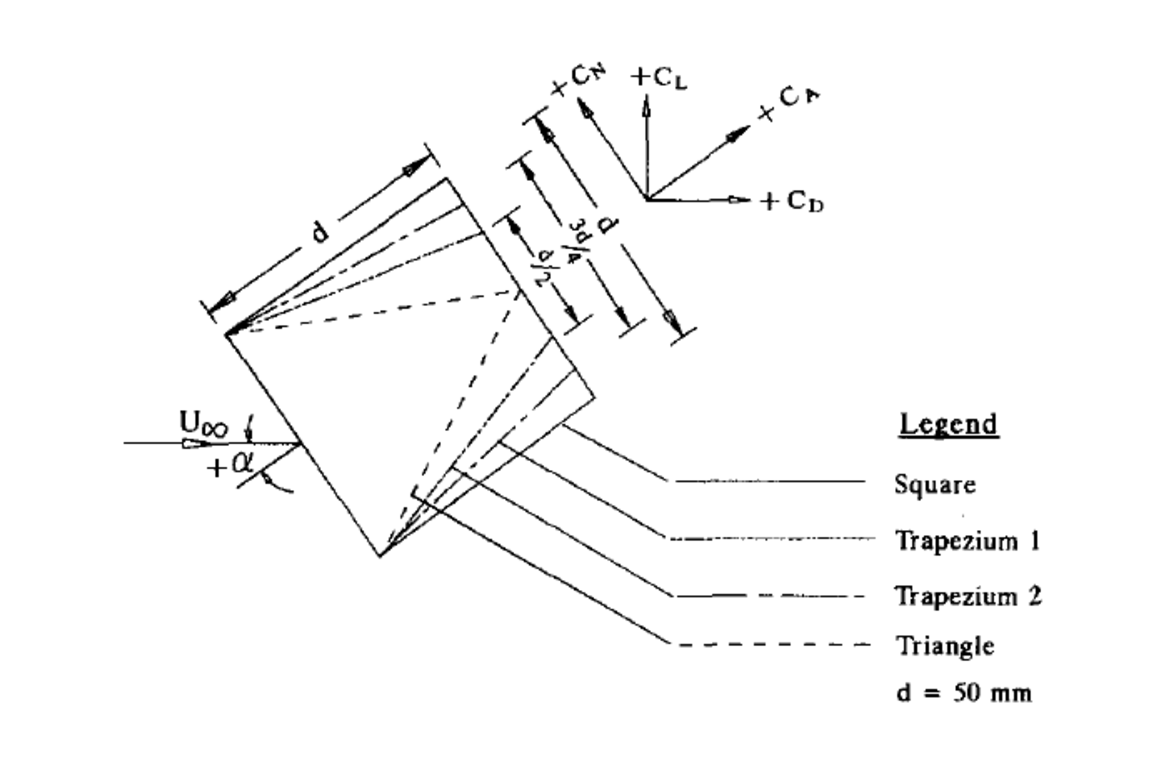
\includegraphics[width=0.75\unitlength]{./fnp/sketch-1.eps}}
     
% 	\put(0.02,0.93){ \large $C_y$} 	
%% 	\put(0.56,1.02){ $\theta$}
% 	
%        \put(0.25,0.8){ $\theta$} 	
%        \put(0.75,0.8){ $\theta$}
%        
%        \put(0.105,1.01){(a)}
%        \put(0.565,1.01){(b)}
     \end{picture}

 }
 \caption{Cross sectional shape considerd in in \cite{Luo2003}}
    \label{fig:lift_curves}
\end{figure}
